\documentclass{../ucll-slides}
\usepackage{../pvm}
\usepackage{fourier}
\usepackage{bbding}

\usetikzlibrary{shadows,shapes.multipart}

\title{Allocation Methods}
\author{Fr\'ed\'eric Vogels}

\newenvironment{procontralist}{
  \begingroup
  \newcommand{\pro}{\item[\Checkmark]}
  \newcommand{\con}{\item[\XSolidBrush]}
  \begin{itemize}
  }{
  \end{itemize}
  \endgroup}


\begin{document}

\begin{frame}
  \titlepage
\end{frame}

\begin{frame}
  \frametitle{Overview}
  \begin{itemize}
    \item Different ways to deal with RAM
    \item Similar to data structures
    \item Trade flexibility for speed
    \item Normally abstracted away as much as possible
    \item In \cpp: crucial to know about the details
  \end{itemize}
\end{frame}

\section{Static Allocation}

\begin{frame}
  \tableofcontents[currentsection]
\end{frame}

\begin{frame}
  \frametitle{Static Allocation}
  \begin{itemize}
    \item Simplest allocation mechanism
    \item Fastest
    \item Most restrictive
    \item Used in oldest programming language \\ (Fortran, early 1950s)
  \end{itemize}
  \vskip1cm
  \begin{center}
    {\color{red}\Huge\danger}
    \parbox{8cm}{\centering 
      {\color{red}\Huge \textsc{warning}} \\
      Examples that follow are what-ifs \\
      They do not show how really \cpp\ works
    }
    {\color{red}\Huge\danger}
  \end{center}
\end{frame}

\begin{frame}
  \frametitle{How Does It Work?}
  \notrealcpp
  \begin{itemize}
    \item The compiler assigns a fixed address to each variable
  \end{itemize}
  \code{allocation.cpp}
  \begin{tikzpicture}[overlay,remember picture,allocation/.style={-latex,thick}]
    \coordinate (upperleft) at (6,4);

    \begin{scope}[scale=.5]
      \coordinate (double) at (upperleft);
      \coordinate (int) at ($ (upperleft) + (0,-1) $);
      \coordinate (char) at ($ (upperleft) + (4,-1) $);

      \visible<2->{
        \draw[fill=red!50] (double) rectangle ++(8,-1);
      }

      \visible<3->{
        \draw[fill=green!50] (int) rectangle ++(4,-1);
      }

      \visible<4->{
        \draw[fill=blue!50] (char) rectangle ++(1,-1);
      }

      \draw (upperleft) grid ++(8,-4);
    \end{scope}

    \visible<2>{
      \draw[allocation] (global) -- (double);
    }

    \visible<3>{
      \draw[allocation] (param) -- ($ (int) + (0,-0.25) $);
    }

    \visible<4>{
      \draw[allocation] (local) -- ($ (char) + (0,-0.25) $);
    }
  \end{tikzpicture}
\end{frame}

\begin{frame}
  \frametitle{Consequences of Static Allocation}
  \notrealcpp
  \begin{itemize}
    \item Compiler needs to have full knowledge at compile-time
  \end{itemize}
  \code{array-creation.cpp}
\end{frame}

\begin{frame}
  \frametitle{Consequences of Static Allocation}
  \notrealcpp
  \begin{itemize}
    \item Local variables ``remember'' their values
  \end{itemize}
  \code{static-locals.cpp}
\end{frame}

\begin{frame}
  \frametitle{Consequences of Static Allocation}
  \notrealcpp
  \begin{itemize}
    \item Recursion not possible
  \end{itemize}
  \code{static-recursion.cpp}
\end{frame}

\begin{frame}
  \frametitle{Static Allocation}
  \begin{procontralist}
    \pro Very fast
    \pro No bookkeeping needed at runtime
    \pro No out-of-memory errors possible
    \pro Entire memory footprint known beforehand
    \con Data structure size must be known at compile time
    \con Full recompilation needed to allow larger data structures
    \con Cannot make use of extra RAM:
         If it's been compiled to work with 1MB but you have 8GB, too bad
    \con No recursion possible
  \end{procontralist}
\end{frame}

\section{Stack Allocation}

\begin{frame}
  \tableofcontents[currentsection]
\end{frame}

\begin{frame}
  \frametitle{Stack Allocation}
  \begin{itemize}
    \item Allocate your variables using static allocation
    \item Introduce a {\tt new} keyword that allows for runtime allocation
    \item Take the remainder of RAM (what's left after static allocation)
    \item Act as if it were a stack of available bytes
    \item Allocation = take top $N$ bytes
  \end{itemize}
  \vskip5mm
  \begin{center}
    \begin{tikzpicture}
      \draw (0,0) rectangle ++(1,2);
      \draw (1,0) rectangle ++(7,2);

      \node[rotate=90] at (0.5,1) {static};
      \node[rotate=90] at (4.5,1) {stack};

      \draw[|-|] (0,-.5) -- ++(8,0) node[midway,below] {RAM};
    \end{tikzpicture}
  \end{center}
\end{frame}

\begin{frame}
  \frametitle{Stack Allocation}
  \notrealcpp
  \begin{columns}
    \column{5cm}
    \code[font size=\small]{stack-allocation.cpp}
    \column{4cm}
    \begin{center}
      \begin{tikzpicture}[allocation/.style={-latex,thick},remember picture,overlay,scale=.5]
        \coordinate (start) at (-4,4);

        \only<3->{
          \draw[fill=red!50] (start) rectangle ++(4,-1);
        }
        \only<3>{
          \draw[allocation] (var a) to [bend left=30] ($ (start) + (0,-0.5) $);
        }

        \only<4->{
          \draw[fill=green!50] ($ (start) + (4,0) $) rectangle ++(4,-1);
        }
        \only<4>{
          \draw[allocation] (var b) to [bend left=30] ($ (start) + (4,-0.5) $);
        }

        \only<5->{
          \draw[fill=blue!50] ($ (start) + (0,-1) $) rectangle ++(4,-1);
        }
        \only<5>{
          \draw[allocation] (var c) to [bend left=30] ($ (start) + (0,-1.5) $);
        }

        \only<6->{
          \draw[fill=yellow!50] ($ (start) + (4,-1) $) rectangle ++(4,-1);
        }
        \only<6>{
          \draw[allocation] (var d) to [bend left=30] ($ (start) + (4,-1.5) $);
        }

        \only<8->{
          \draw[fill=red!50] ($ (start) + (0,-2) $) rectangle ++(8,-2);
        }
        \only<8>{
          \draw[allocation] (mem a) to [bend right=30] ($ (start) + (0,-2.5) $);
        }

        \only<9->{
          \draw[fill=green!50] ($ (start) + (0,-4) $) rectangle ++(8,-3);
        }
        \only<9>{
          \draw[allocation] (mem b) to [bend right=30] ($ (start) + (0,-4.5) $);
        }

        \only<10->{
          \draw[fill=blue!50] ($ (start) + (0,-7) $) rectangle ++(4,-1);
        }
        \only<10>{
          \draw[allocation] (mem c) to [bend right=30] ($ (start) + (0,-7.5) $);
        }

        \only<11->{
          \draw[fill=yellow!50] ($ (start) + (4,-7) $) rectangle ++(4,-1);
          \draw[fill=yellow!50] ($ (start) + (0,-8) $) rectangle ++(8,-1);
        }
        \only<11>{
          \draw[allocation] (mem d) to [bend right=30] ($ (start) + (4,-7.5) $);
        }

        \draw (start) grid ++(8,-9);
      \end{tikzpicture}
    \end{center}
  \end{columns}
  \vskip2cm
  \begin{overprint}
    \onslide<2-6>
    \begin{center}
      \textbf{Compilation stage} \\ Compiler assigns memory locations to each variable \\ (this is still static allocation)
    \end{center}
    \onslide<7->
    \begin{center}
      \textbf{At runtime} \\ Extra memory is allocated on stack at runtime
    \end{center}
  \end{overprint}
\end{frame}

\begin{frame}
  \frametitle{Stack Allocation}
  \begin{itemize}
    \item You can keep on allocating\dots
    \item \dots but eventually you'll run out of memory
    \item Why not deallocate unused memory?
    \item Problem: can only deallocate what's on top of the stack
  \end{itemize}
  \code[font size=\small,width=6cm]{stack-deallocation.cpp}
\end{frame}

\begin{frame}
  \frametitle{Stack Allocation}
  \begin{procontralist}
    \pro Fast allocation
    \pro Little runtime bookkeeping needed
    \pro Can allocate any amount of memory you want at runtime
    \pro Recursion made possible
    \con Problematic deallocation
  \end{procontralist}
\end{frame}

\section{Heap Allocation}

\begin{frame}
  \tableofcontents[currentsection]
\end{frame}

\begin{frame}
  \frametitle{Heap Allocation}
  \begin{itemize}
    \item Step 1: use static allocation where possible
    \item Step 2: pick part of RAM and declare it stack
    \item Step 3: remainder of RAM is heap
  \end{itemize}
  \vskip5mm
  \begin{center}
    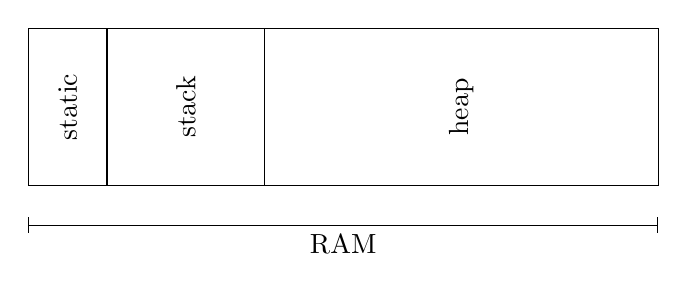
\begin{tikzpicture}
      \draw (0,0) rectangle ++(1,2);
      \draw (1,0) rectangle ++(2,2);
      \draw (3,0) rectangle ++(5,2);

      \node[rotate=90] at (0.5,1) {static};
      \node[rotate=90] at (2,1) {stack};
      \node[rotate=90] at (5.5,1) {heap};

      \draw[|-|] (0,-.5) -- ++(8,0) node[midway,below] {RAM};
    \end{tikzpicture}
  \end{center}
\end{frame}

\begin{frame}
  \frametitle{Heap Allocation}
  \notrealcpp
  \begin{columns}
    \column{5cm}
    \code[font size=\small]{heap-allocation.cpp}
    \column{4cm}
    \begin{center}
      \begin{tikzpicture}[allocation/.style={-latex,thick},remember picture,overlay,scale=.5]
        \coordinate (start) at (-4,4);

        \only<3->{
          \draw[fill=red!50] (start) rectangle ++(4,-1);
        }
        \only<3>{
          \draw[allocation] (var a) to [bend left=30] ($ (start) + (0,-.5) $);
        }

        \only<4->{
          \draw[fill=green!50] ($ (start) + (4,0) $) rectangle ++(4,-1);
        }
        \only<4>{
          \draw[allocation] (var b) to [bend left=30] ($ (start) + (4,-0.5) $);
        }

        \only<5->{
          \draw[fill=blue!50] ($ (start) + (0,-1) $) rectangle ++(4,-1);
        }
        \only<5>{
          \draw[allocation] (var c) to [bend left=30] ($ (start) + (0,-1.5) $);
        }

        \only<6->{
          \draw[fill=yellow!50] ($ (start) + (4,-1) $) rectangle ++(4,-1);
        }
        \only<6>{
          \draw[allocation] (var d) to [bend left=30] ($ (start) + (4,-1.5) $);
        }

        \only<7-11>{
          \draw[fill=red!50] ($ (start) + (0,-2) $) rectangle ++(8,-1);
        }
        \only<7>{
          \draw[allocation] (mem a) to [bend right=30] ($ (start) + (0,-2.5) $);
        }

        \only<8-10>{
          \draw[fill=green!50] ($ (start) + (0,-3) $) rectangle ++(8,-3);
        }
        \only<8>{
          \draw[allocation] (mem b) to [bend right=30] ($ (start) + (0,-3.5) $);
        }

        \only<9-12>{
          \draw[fill=blue!50] ($ (start) + (0,-6) $) rectangle ++(8,-2);
        }
        \only<9>{
          \draw[allocation] (mem b) to [bend right=30] ($ (start) + (0,-6.5) $);
        }

        \only<10-13>{
          \draw[fill=yellow!50] ($ (start) + (0,-8) $) rectangle ++(8,-2);
        }
        \only<10>{
          \draw[allocation] (mem d) to [bend right=30] ($ (start) + (0,-8.5) $);
        }

        \only<11>{
          \draw[->,thick] (del b) ++(2,0) -- ++(-1,0);
        }

        \only<12>{
          \draw[->,thick] (del a) ++(2,0) -- ++(-1,0);
        }

        \only<13>{
          \draw[->,thick] (del c) ++(2,0) -- ++(-1,0);
        }

        \only<14>{
          \draw[->,thick] (del d) ++(2,0) -- ++(-1,0);
        }

        \draw (start) grid ++(8,-10);
      \end{tikzpicture}
    \end{center}
  \end{columns}
  \vskip2cm
  \begin{overprint}
    \onslide<2-6>
    \begin{center}
      \textbf{Compilation stage} \\ Compiler assigns memory locations to each variable \\ (this is still static allocation)
    \end{center}

    \onslide<7->
    \begin{center}
      \textbf{At runtime}
    \end{center}
  \end{overprint}
\end{frame}

\begin{frame}
  \frametitle{Heap Allocation}
  \begin{procontralist}
    \pro Allows allocation of arbitrarily large blocks
    \pro Deallocation possible in any order
    \pro Most general allocation method
    \con Requires some bookkeeping \\ (keeps track of linked list of free blocks)
    \con Allocation/Deallocation relatively slow
    \con Fragmentation
  \end{procontralist}
\end{frame}

%    \item Generally used for function-local data


\end{document}